% THIS DOCUMENT IS TAILORED TO REQUIREMENTS FOR SCIENTIFIC COMPUTING.  IT SHOULDN'T
% BE USED FOR NON-SCIENTIFIC COMPUTING PROJECTS
\documentclass[12pt]{article}

\usepackage{amsmath, mathtools}
\usepackage{amsfonts}
\usepackage{amssymb}
\usepackage{graphicx}
\usepackage{colortbl}
\usepackage{xr}
\usepackage{hyperref}
\usepackage{longtable}
\usepackage{xfrac}
\usepackage{tabularx}
\usepackage{float}
\usepackage{siunitx}
\usepackage{booktabs}
\usepackage{caption}
\usepackage{pdflscape}
\usepackage{afterpage}

\usepackage[round]{natbib}

%\usepackage{refcheck}

\hypersetup{
    bookmarks=true,         % show bookmarks bar?
      colorlinks=true,       % false: boxed links; true: colored links
    linkcolor=red,          % color of internal links (change box color with linkbordercolor)
    citecolor=green,        % color of links to bibliography
    filecolor=magenta,      % color of file links
    urlcolor=cyan           % color of external links
}

%% Comments

\usepackage{color}

\newif\ifcomments\commentstrue %displays comments
%\newif\ifcomments\commentsfalse %so that comments do not display

\ifcomments
\newcommand{\authornote}[3]{\textcolor{#1}{[#3 ---#2]}}
\newcommand{\todo}[1]{\textcolor{red}{[TODO: #1]}}
\else
\newcommand{\authornote}[3]{}
\newcommand{\todo}[1]{}
\fi

\newcommand{\wss}[1]{\authornote{blue}{SS}{#1}} 
\newcommand{\plt}[1]{\authornote{magenta}{TPLT}{#1}} %For explanation of the template
\newcommand{\an}[1]{\authornote{cyan}{Author}{#1}}

%% Common Parts

\newcommand{\progname}{Optimal EM Placement} % PUT YOUR PROGRAM NAME HERE
\newcommand{\authname}{Hussein Saad} % AUTHOR NAMES                  

\usepackage{hyperref}
    \hypersetup{colorlinks=true, linkcolor=blue, citecolor=blue, filecolor=blue,
                urlcolor=blue, unicode=false}
    \urlstyle{same}
                                


% For easy change of table widths
\newcommand{\colZwidth}{1.0\textwidth}
\newcommand{\colAwidth}{0.13\textwidth}
\newcommand{\colBwidth}{0.82\textwidth}
\newcommand{\colCwidth}{0.1\textwidth}
\newcommand{\colDwidth}{0.05\textwidth}
\newcommand{\colEwidth}{0.8\textwidth}
\newcommand{\colFwidth}{0.17\textwidth}
\newcommand{\colGwidth}{0.5\textwidth}
\newcommand{\colHwidth}{0.28\textwidth}

% Used so that cross-references have a meaningful prefix
\newcounter{defnum} %Definition Number
\newcommand{\dthedefnum}{GD\thedefnum}
\newcommand{\dref}[1]{GD\ref{#1}}
\newcounter{datadefnum} %Datadefinition Number
\newcommand{\ddthedatadefnum}{DD\thedatadefnum}
\newcommand{\ddref}[1]{DD\ref{#1}}
\newcounter{theorynum} %Theory Number
\newcommand{\tthetheorynum}{TM\thetheorynum}
\newcommand{\tref}[1]{TM\ref{#1}}
\newcounter{tablenum} %Table Number
\newcommand{\tbthetablenum}{TB\thetablenum}
\newcommand{\tbref}[1]{TB\ref{#1}}
\newcounter{assumpnum} %Assumption Number
\newcommand{\atheassumpnum}{A\theassumpnum}
\newcommand{\aref}[1]{A\ref{#1}}
\newcounter{goalnum} %Goal Number
\newcommand{\gthegoalnum}{GS\thegoalnum}
\newcommand{\gsref}[1]{GS\ref{#1}}
\newcounter{instnum} %Instance Number
\newcommand{\itheinstnum}{IM\theinstnum}
\newcommand{\iref}[1]{IM\ref{#1}}
\newcounter{reqnum} %Requirement Number
\newcommand{\rthereqnum}{R\thereqnum}
\newcommand{\rref}[1]{R\ref{#1}}
\newcounter{nfrnum} %NFR Number
\newcommand{\rthenfrnum}{NFR\thenfrnum}
\newcommand{\nfrref}[1]{NFR\ref{#1}}
\newcounter{lcnum} %Likely change number
\newcommand{\lthelcnum}{LC\thelcnum}
\newcommand{\lcref}[1]{LC\ref{#1}}

\usepackage{fullpage}
\usepackage{bm}

\newcommand{\deftheory}[9][Not Applicable]
{
\newpage
\noindent \rule{\textwidth}{0.5mm}

\paragraph{RefName: } \textbf{#2} \phantomsection 
\label{#2}

\paragraph{Label:} #3

\noindent \rule{\textwidth}{0.5mm}

\paragraph{Equation:}

#4

\paragraph{Description:}

#5

\paragraph{Notes:}

#6

\paragraph{Source:}

#7

\paragraph{Ref.\ By:}

#8

\paragraph{Preconditions for \hyperref[#2]{#2}:}
\label{#2_precond}

#9

\paragraph{Derivation for \hyperref[#2]{#2}:}
\label{#2_deriv}

#1

\noindent \rule{\textwidth}{0.5mm}

}

\begin{document}

\title{Software Requirements Specification for \progname: Convex Optimization for Optimal Positioning of Electromagnetic Actuators} 
\author{\authname}
\date{\today}
	
\maketitle

~\newpage

\pagenumbering{roman}

\tableofcontents

~\newpage

\section*{Revision History}

\begin{tabularx}{\textwidth}{p{3cm}p{2cm}X}
\toprule {\bf Date} & {\bf Version} & {\bf Notes}\\
\midrule
\today & 1.0 & First draft\\
\bottomrule
\end{tabularx}


~\newpage

\section{Reference Material}

This section records information for easy reference.

\subsection{Table of Units}

Throughout this document SI (Syst\`{e}me International d'Unit\'{e}s) is employed
as the unit system.  In addition to the basic units, several derived units are
used as described below.  For each unit, the symbol is given followed by a
description of the unit and the SI name.
~\newline

\renewcommand{\arraystretch}{1.2}
%\begin{table}[ht]
  \noindent \begin{tabular}{l l l} 
    \toprule		
    \textbf{symbol} & \textbf{unit} & \textbf{SI}\\
    \midrule 
    \si{\metre} & length & metre\\
    \si{\ampere} & current & ampere\\
    \si{\newton} & force & newton\\
    \si{\tesla} & magnetic flux density & tesla\\
    \bottomrule
  \end{tabular}
  %	\caption{Provide a caption}
%\end{table}

\subsection{Table of Symbols}

The table that follows summarizes the symbols used in this document along with
their units.  The choice of symbols was made to be consistent with existing literature around magnetic actuation systems.

\renewcommand{\arraystretch}{1.2}
%\noindent \begin{tabularx}{1.0\textwidth}{l l X}
\noindent \begin{longtable*}{l l p{12cm}} \toprule
\textbf{symbol} & \textbf{unit} & \textbf{description}\\
\midrule 
$N$ & - & number of turns in a coil
\\
$i$ & \si{\ampere} & current received by one coil
\\
$A$ & \si{\metre}$^2$ & cross-sectional area of one coil
\\
$M$ & - & sample size
\\
$K$ & - & desired number of electromagnets 
\\
$V$ & \si{\metre}$^3$ & allocated under-the-table volume
\\
$t$ & \si{\metre} & target location
\\
\bottomrule
\end{longtable*}


\subsection{Abbreviations and Acronyms}

\renewcommand{\arraystretch}{1.2}
\begin{tabular}{l l} 
  \toprule		
  \textbf{symbol} & \textbf{description}\\
  \midrule 
  A & Assumption\\
  DD & Data Definition\\
  GD & General Definition\\
  GS & Goal Statement\\
  IM & Instance Model\\
  LC & Likely Change\\
  PS & Physical System Description\\
  R & Requirement\\
  SRS & Software Requirements Specification\\
  TM & Theoretical Model\\
  EM & Electromagnet \\
  \bottomrule
\end{tabular}\\


\subsection{Mathematical Notation}
Vectors and matrices are bolded to fit the \hyperlink{https://journals.ieeeauthorcenter.ieee.org/your-role-in-article-production/ieee-editorial-style-manual/}{IEEE typesetting guide}.

\newpage

\pagenumbering{arabic}
\section{Introduction}
Microrobots hold immense promise for a variety of clinical and surgical procedures. Their size and wireless
controllability allow them to navigate complex and tortuous area of the human body with minimal collateral damage. However,
clinical adoption of these devices is hurdled by complexities in the actuation systems that control them \cite{bozuyuk2024roadmap}. Magnetic actuation is 
perhaps the most common method of manipulating these devices, as magnetic fields can safely penetrate the human body and offer a high level of controllability. Magnetic fields can be generated through either EMs
or permanent magnets, and while the latter offer higher stronger magnetic fields, EM coils are generally preferred
because their magnetic field strength can be regulated by adjusting their power input~\cite{hwang2020review}. However, EMs tend to be bulky and can potentially obstruct a clinician's access to the workspace. Even with recent designs that place the actuation system under the operating table, generating magnetic fields large enough to cover a patient-sized workspace remains a challenge. 

We propose a convex optimization algorithm to solve the optimal EM arrangement problem for under-the-table actuation systems. Our program solves for the positions of EM actuators that yield the highest system manipulability. 

This section explains the purpose of the document, the scope of requirements, the characteristics of the intended reader and the organization of the document.

\subsection{Purpose of Document}
The purpose of this document is to describe the mathematical methods used in solving the optimal EM arrangement problem. Thus, it is to be used as a reference to all information necessary for people who wish to verify or contribute to the software. 


\subsection{Scope of Requirements} 
The scope of the requirements is to present the mathematical models used in determining the optimal poses of electromagnetics in an under-the-table actuation system. The models used do not claim the optimality of any metrics other than positional and orientational metrics of EMs.   


\subsection{Characteristics of Intended Reader} \label{sec_IntendedReader}
The Intended Reader of this document must possess an understanding of magnetism at the first-year university level. In addition, a solid foundation in linear algebra at the freshman level is required. The reader should also have cursory knowledge of optimization.

\subsection{Organization of Document}
The SRS follows a standard pattern of presenting background knowledge, goals, definitions, assumptions, theories, and instance models. Readers who are familiar with the information presented in theoretical models may want to skip to the instance models section and refer back to earlier information as needed. 


\section{General System Description}

This section provides general information about the system.  It identifies the
interfaces between the system and its environment, describes the user
characteristics and lists the system constraints.

\subsection{System Context} \label{Sec_SysContext}
As the system context shows in the below figure, the user, represented by the circle, is responsible for both program inputs and outputs. The program itself is represented by the box, and the flow of information is indicated by the direction of the arrows. 

\begin{figure}[h!]
\begin{center}
 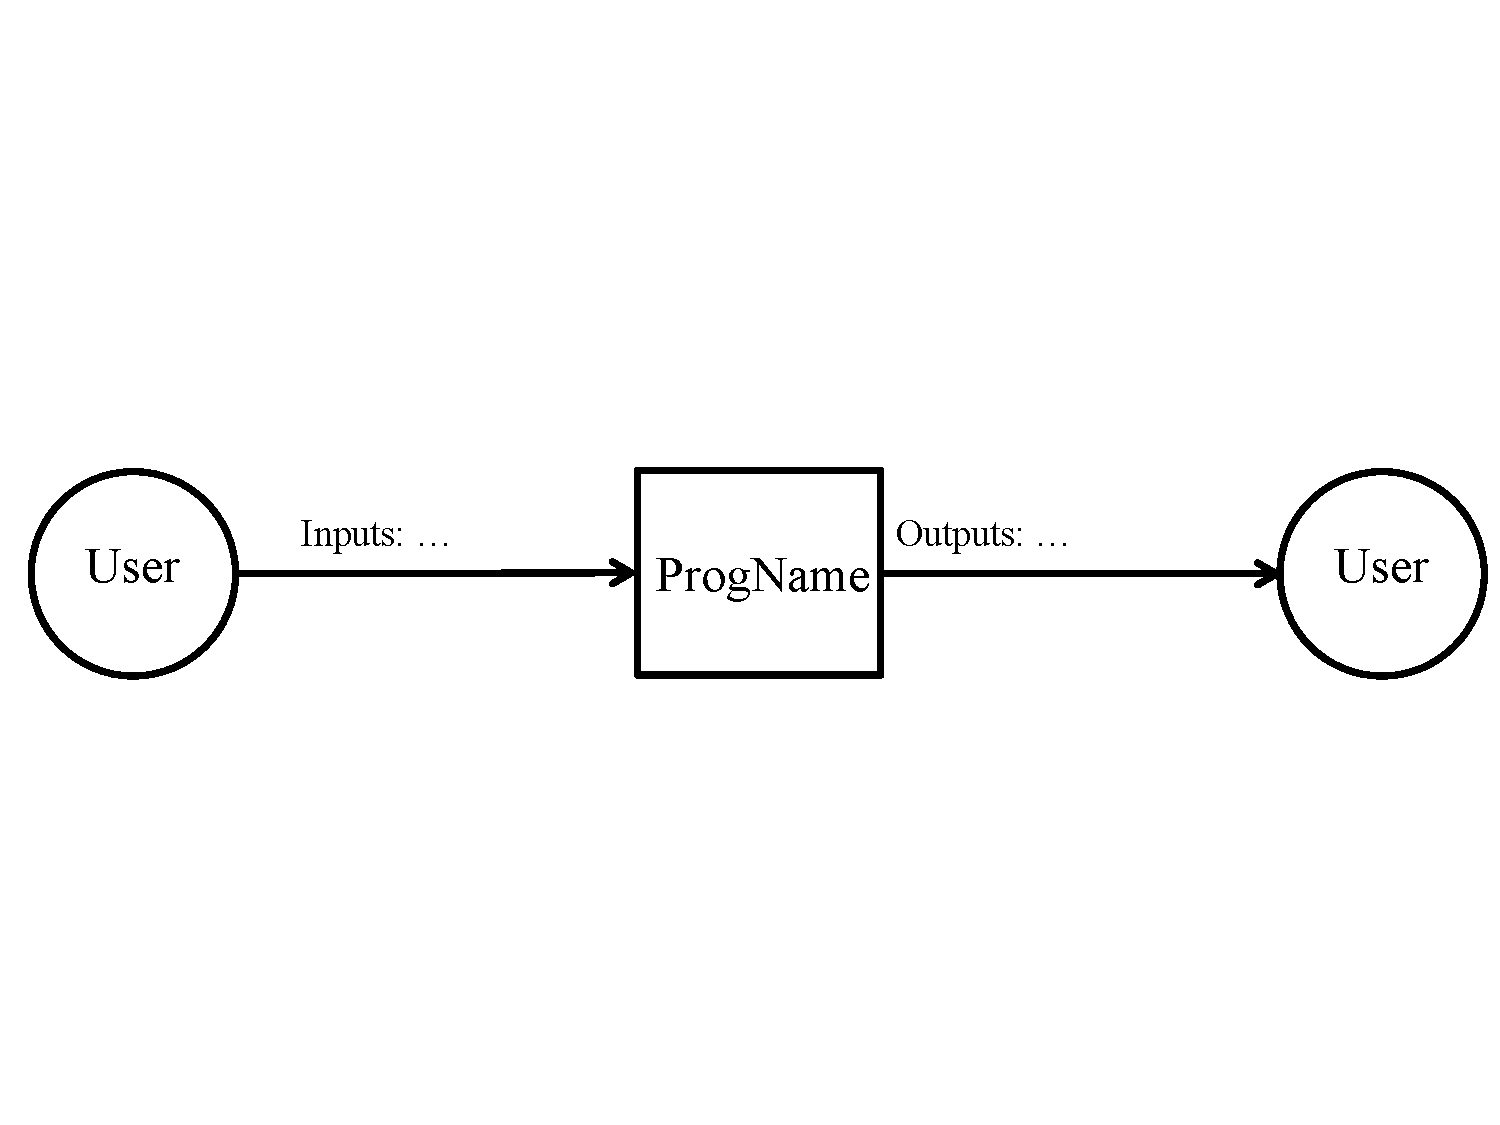
\includegraphics[width=0.6\textwidth]{SystemContextFigure}
\caption{System Context}
\label{Fig_SystemContext} 
\end{center}
\end{figure}
\begin{itemize}
\item User Responsibilities:
\begin{itemize}
\item Provide the required input including EM geometry, under-the-table volume, sample size and desired number of EMs. 
\item Ensure all inputs are valid.
\end{itemize}
\item \progname{} Responsibilities:
\begin{itemize}
\item Detect data type mismatch, such as a string of characters instead of a
  floating point number.
\item Determine the most optimal poses of the desired number of EMs within the under-the-table volume. 
\item Ensure that the arrangement is physically feasible. 
\end{itemize}
\end{itemize}

The program is typically used in two settings: engineering and scientific research. In engineering, it is primarily used during the planning phase and is not integrated into live systems. Thus, it is neither safety-critical nor mission-critical.

\subsection{User Characteristics} \label{SecUserCharacteristics}
The end user of the system is expected to be familiar with elementary magnetism concepts. 

\subsection{System Constraints}
This project has no system constraints. 

\section{Specific System Description}
This section first presents the problem description, which gives a high-level
view of the problem to be solved.  This is followed by the solution characteristics
specification, which presents the assumptions, theories, definitions and finally
the instance models. 

\subsection{Problem Description} \label{Sec_pd}
\progname{} is intended to solve the optimal magnet arrangement problem for under-the-table EM actuation systems. 

\subsubsection{Terminology and  Definitions}
This subsection provides a list of terms that are used in the subsequent
sections and their meaning, with the purpose of reducing ambiguity and making it
easier to correctly understand the requirements:

\begin{itemize}
\item Microrobot: A robot with dimensions less than 1mm. 
\item Pose: A position in 3D space together with an angular configuration.
\item Workspace: The space encompassed by the magnetic fields generated by the EMs.
\item Magnetic actuation: The use of magnetic fields to wirelessly manipulate an object.
\item Solenoid: A type of EM formed by a helical coil of wire whose length is significantly greater than its diameter. 
\end{itemize}

\subsubsection{Physical System Description} \label{sec_phySystDescrip}
The physical system of \progname{} includes the following elements:
\begin{itemize}
\item[PS1:] An operating table.
\item[PS2:] A set amount of cubic volume available under the operating table.
\item[PS3:] Some number of EMs.  
\end{itemize}

\subsubsection{Goal Statements}
\noindent Given the volume of the under-the-table space, the size of the EMs (number of turns, area), the current received by the system, a target location, the desired number of EMs, and sample size, the goal statements are:
\begin{itemize}
\item[GS\refstepcounter{goalnum}\thegoalnum \label{G_1}:] Calculate the positions of the EMs that maximize the manipulability over the workspace.
\item[GS\refstepcounter{goalnum}\thegoalnum \label{G_meaningfulLabel}:] Calculate the magnetic force and torque values at the target location.
\end{itemize}

\subsection{Solution Characteristics Specification}
\begin{figure}[H]
  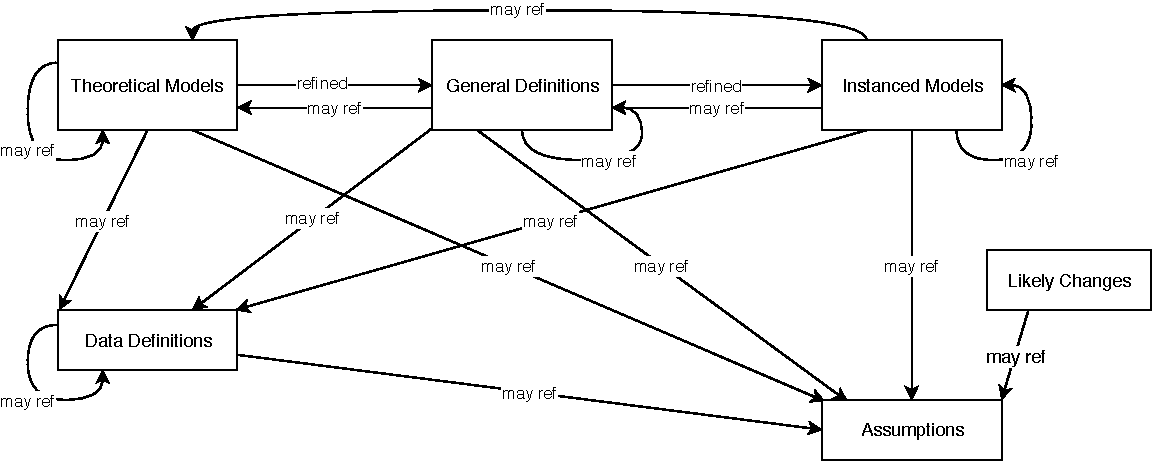
\includegraphics[scale=0.9]{RelationsBetweenTM_GD_IM_DD_A.pdf}
\end{figure}
The instance models that govern \progname{} are presented in
Subsection~\ref{sec_instance}.  The information to understand the meaning of the
instance models and their derivation is also presented, so that the instance
models can be verified.

\subsubsection{Assumptions} \label{sec_assumpt}
This section simplifies the original problem and helps in developing the
theoretical model by filling in the missing information for the physical system.
The numbers given in the square brackets refer to the theoretical model [TM],
general definition [GD], data definition [DD], or instance model [IM], in which the respective assumption is used.
\begin{itemize}
\item[A\refstepcounter{assumpnum}\theassumpnum \label{a_current}:] All EMs are receiving the same, constant current. 
\item[A\refstepcounter{assumpnum}\theassumpnum \label{a_geom}:] All EMs are identical in geometric properties. 
\item[A\refstepcounter{assumpnum}\theassumpnum \label{a_cyl}:] All EMs are perfectly cylindrical.
\item[A\refstepcounter{assumpnum}\theassumpnum \label{solenoid_a}:] All EMs follow the solenoid model.
\end{itemize}

\subsubsection{Theoretical Models}\label{sec_theoretical}
This section focuses on the general equations and laws that \progname{} is based on.
~\newline

\noindent
\begin{minipage}{\textwidth}
\renewcommand*{\arraystretch}{1.5}
\begin{tabular}{| p{\colAwidth} | p{\colBwidth}|}
  \hline
  \rowcolor[gray]{0.9}
  Number& TM\refstepcounter{theorynum}\thetheorynum \label{TM_1}\\
  \hline
  Label& \bf Magnetic Moment of a Solenoid\\
  \hline
  Equation &
    $m = NiA$ \\ 
  \hline
  Description
    & The above equation calculates the magnetic moment of a solenoid EM.  \\
  
   & $N$ is the number of turns in the coil.  \\
  
  & $i$ is the current received by the solenoid (A).  \\
  
  & $A$ is the cross-sectional area of the solenoid ($m^2$). \\
  \hline
  Notes & - \\
  \hline
  Sources& \url{https://en.wikipedia.org/wiki/Magnetic_moment} \\
  \hline
  Ref.\ By &  TM\ref{TM_2} \\
  \hline
\end{tabular}
\end{minipage}\\
~\newline


\noindent
\begin{minipage}{\textwidth}
\renewcommand*{\arraystretch}{1.5}
\begin{tabular}{| p{\colAwidth} | p{\colBwidth}|}
  \hline
  \rowcolor[gray]{0.9}
  Number& TM\refstepcounter{theorynum}\thetheorynum \label{TM_2}\\
  \hline
  Label& \bf Magnetic Field of a Magnetic Moment\\
  \hline
  Equation &
    $\bm B (\bm p) = \frac{\mu_0 \vert \vert  \bm m \vert \vert }
  {4\pi \vert \vert  \bm r \vert \vert^3} 
  (3 \hat{\bm r} \hat{\bm r}^{\top} - \mathbb{I}) \hat{\bm m}$ \\ 
  \hline
  Description
    & The magnetic field at some point $\bm p$ can be calculated using the equation above.  \\
  
   & $\mu_0 = 4\pi \times 10^{-7}$ Tm/A is the permeability of free space.  \\
  
  & $\bm r$ is the position of the point relative to the center of the magnet (m). $\hat{\bm r}$ is the unit vector of $r$.  \\
  
  & $\bm m$ is the magnetic moment of magnet generating the field (T). \\
  & $\mathbb{I}$ is the identity matrix. \\
  \hline
  Notes & - \\
  \hline
  Sources& \url{https://en.wikipedia.org/wiki/Magnetic_moment} \\
  \hline
  Ref.\ By &  TM\ref{TM_3}, IM\ref{umat} \\
  \hline
\end{tabular}
\end{minipage}\\
~\newline

\noindent
\begin{minipage}{\textwidth}
\renewcommand*{\arraystretch}{1.5}
\begin{tabular}{| p{\colAwidth} | p{\colBwidth}|}
  \hline
  \rowcolor[gray]{0.9}
  Number& TM\refstepcounter{theorynum}\thetheorynum \label{TM_3}\\
  \hline
  Label& \bf Magnetic Force on a Magnetized Object\\
  \hline
  Equation &
    $\bm F = \nabla (\bm m \cdot \bm B)$ \\ 
  \hline
  Description
    & The force experienced by some magnetized object with magnetic moment $m$ can be found as presented.  \\
  
   & $\nabla$ is the field gradient.  \\
  
  & $\bm m$ is the magnetic moment of the object (T).  \\
  
  & $\bm B$ is the magnetic field the object is in. \\
  \hline
  Notes & - \\
  \hline
  Sources& \url{https://en.wikipedia.org/wiki/Magnetic_field} \\
  \hline
  Ref.\ By &  IM\ref{umat} \\
  \hline
\end{tabular}
\end{minipage}\\
~\newline

\noindent
\begin{minipage}{\textwidth}
\renewcommand*{\arraystretch}{1.5}
\begin{tabular}{| p{\colAwidth} | p{\colBwidth}|}
  \hline
  \rowcolor[gray]{0.9}
  Number& TM\refstepcounter{theorynum}\thetheorynum \label{TM_4}\\
  \hline
  Label& \bf Manipulator Jacobian\\
  \hline
  Equation &
    $\bm J(x) = \begin{bmatrix}
    \bm J_v(x) \\
    \bm J_w(x)
  \end{bmatrix}$ \\ 
  \hline
  Description
    & The relationship between the inputs and outputs of a robotic system can be described by a Jacobian.  \\
  
   & $\bm J_{v,w}$ are the Jacobians describing an output $v, w$ respectively.  \\
  \hline
  Notes & - \\
  \hline
  Sources& Robotic Modeling and Control by Mark Spong. \\
  \hline
  Ref.\ By &  IM\ref{umat} \\
  \hline
\end{tabular}
\end{minipage}\\
~\newline

\noindent
\begin{minipage}{\textwidth}
\renewcommand*{\arraystretch}{1.5}
\begin{tabular}{| p{\colAwidth} | p{\colBwidth}|}
  \hline
  \rowcolor[gray]{0.9}
  Number& TM\refstepcounter{theorynum}\thetheorynum \label{TM_5}\\
  \hline
  Label& \bf Robotic Manipulability\\
  \hline
  Equation &
    $\mu \triangleq \prod_{i=1}^{n} \sigma_i \propto \sqrt{det(\bm J \bm J^\top)}$ \\ 
  \hline
  Description
    & The manipulability of a robotic system is given by the product of singular values of its Jacobian. \\
  
   & $\sigma_i$ is the $i$-th singular value of the system.  \\
   & $\bm J$ is the Jacobian of the system with respect to some input.  \\
  \hline
  Notes & - \\
  \hline
  Sources& Robotic Modeling and Control by Mark Spong. \\
  \hline
  Ref.\ By &  IM\ref{obj_fun} \\
  \hline
\end{tabular}
\end{minipage}\\

\subsubsection{Data Definitions}\label{sec_datadef}
This section collects and defines all the data needed to build the instance
models. The dimension of each quantity is also given.

~\newline

\noindent
\begin{minipage}{\textwidth}
\renewcommand*{\arraystretch}{1.5}
\begin{tabular}{| p{\colAwidth} | p{\colBwidth}|}
\hline
\rowcolor[gray]{0.9}
Number& DD\refstepcounter{datadefnum}\thedatadefnum \label{perm_vac}\\
\hline
Label& \bf Permeability of Free Space\\
\hline
Symbol &$\mu_0$\\
\hline
% Units& $Mt^{-3}$\\
% \hline
  SI Units & \si{\tesla\metre\per\ampere}\\
  \hline
  Equation& $\mu_0 = 4\pi \times 10^{-7} \text{ }\si{\tesla\metre\per\ampere}$\\
  \hline
  Description & 
  Permeability is the measure of magnetization produced in a material in response to an applied magnetic field. Above the permeability of material in free space (vacuum).
  \\
  \hline
  Sources& \url{https://en.wikipedia.org/wiki/Vacuum_permeability} \\
  \hline
  Ref.\ By & TM\ref{TM_2}\\
  \hline
\end{tabular}
\end{minipage}\\

\newpage

\subsubsection{Instance Models} \label{sec_instance}    
This section transforms the problem defined in Section~\ref{Sec_pd} into 
one which is expressed in mathematical terms. It uses concrete symbols defined 
in Section~\ref{sec_datadef} to replace the abstract symbols in the models 
identified in Sections~\ref{sec_theoretical}. The goal G~\ref{G_1} is solved by IM~\ref{obj_fun}. 

~\newline


\noindent
\begin{minipage}{\textwidth}
\renewcommand*{\arraystretch}{1.5}
\begin{tabular}{| p{\colAwidth} | p{\colBwidth}|}
\hline
\rowcolor[gray]{0.9}
Number& IM\refstepcounter{instnum}\theinstnum \label{umat}\\
\hline
Label &\bf Actuation Matrix \\
\hline
Equation&$ \mathcal{\bm U} = \begin{bmatrix}
  \bm B \\ \bm F
\end{bmatrix}$  \\
\hline
Description &
The actuation matrix is an example of a Jacobian manipulator the relies on Magnetic field and Force values. 
\\
& $\bm B$ and $\bm F$ are the matrices containing magnetic field and force values.
\\
\hline
  Source & - \\
  \hline
  Ref.\ By & IM\ref{obj_fun} \\
  \hline
\end{tabular}
\end{minipage}\\

~\newline
%Instance Model 1

\noindent
\begin{minipage}{\textwidth}
\renewcommand*{\arraystretch}{1.5}
\begin{tabular}{| p{\colAwidth} | p{\colBwidth}|}
  \hline
  \rowcolor[gray]{0.9}
  Number& IM\refstepcounter{instnum}\theinstnum \label{obj_fun}\\
  \hline
  Label& \bf Objective Function $f(x)$\\
  \hline
  Input&$\mathcal{\bm U}$, $M$, $K$\\
  \hline
  Output& $\bm x \in \{0,1\}^K$ s.t. $\bm 1_M^\top \bm x = K$ and $f(x) = \sum_{i=1}^{K}\bm x_i \bm U_i \bm U_i^\top$ is maximized \\
  \hline
  Description&$\mathcal{\bm U}$ is the actuation matrix.\\
  &$M$ and $K$ are the sample size and desired number of EMs.
  \\
  \hline
  Sources& - \\
  \hline
  Ref.\ By & -\\
  \hline
\end{tabular}
\end{minipage}\\

\subsubsection{Input Data Constraints} \label{sec_DataConstraints}    
Table~\ref{TblInputVar} shows the data constraints on the input output
variables.  The column for physical constraints gives the physical limitations
on the range of values that can be taken by the variable.  The column for
software constraints restricts the range of inputs to reasonable values.  The
software constraints will be helpful in the design stage for picking suitable
algorithms.  The constraints are conservative, to give the user of the model the
flexibility to experiment with unusual situations.  The column of typical values
is intended to provide a feel for a common scenario.  The uncertainty column
provides an estimate of the confidence with which the physical quantities can be
measured.  This information would be part of the input if one were performing an
uncertainty quantification exercise.

\begin{table}[!h]
  \caption{Input Variables} \label{TblInputVar}
  \renewcommand{\arraystretch}{1.2}
\noindent \begin{longtable*}{l l l l c} 
  \toprule
  \textbf{Var} & \textbf{Physical Constraints} & \textbf{Software Constraints} &
                             \textbf{Typical Value} & \textbf{Uncertainty}\\
  \midrule 
  $N$ & $N > 0$ & $0 < N \leq \text{int}_{\text{max}}$ & 100 & 0\%
  \\
  $I$ & $I > 0$ & $0 < I \leq 20000 \text{A}$ & 10A & 10\%
  \\
  $A$ & $A > 0$ & $A > 0$ & 6m$^2$ & 5\%
  \\
  $M$ & $M > 0$ & $0 < M < \text{int}_\text{max}$ & 10000 & 0\%
  \\
  $K$ & $0 < K < M$ & $0 < K < \text{int}_\text{max}$ & 8 & 0\%
  \\
  $V$ & $V > 0$ & $V > 0$ & 1m$^3$ & 0\%
  \\
  $t$ & $t > 0$ & $t > 0$ & 0.1m & 10\%
  \\
  \bottomrule
\end{longtable*}
\end{table}

\subsubsection{Properties of a Correct Solution} \label{sec_CorrectSolution}

\noindent
A correct solution must exhibit the properties stated in Table~\ref{TblOutputVar}

\begin{table}[!h]
\caption{Output Variables} \label{TblOutputVar}
\renewcommand{\arraystretch}{1.2}
\noindent \begin{longtable*}{l l} 
  \toprule
  \textbf{Var} & \textbf{Physical Constraints} \\
  \midrule 
  $\bm x$ & $\sum_{i=1}^{M} \bm x_i = K$
  \\
  \bottomrule
\end{longtable*}
\end{table}


\section{Requirements}
This section provides the functional requirements, the tasks that the
software is expected to complete, and the non-functional requirements, the
qualities that the software is expected to possess.

\subsection{Functional Requirements}

\noindent \begin{itemize}

\item[R\refstepcounter{reqnum}\thereqnum \label{R_Inputs}:] Provide the inputs specific to EMs (number of turns, cross-sectional area, current), and actuation system (number of samples and actuators, volume) and a target location. 
\item[R\refstepcounter{reqnum}\thereqnum \label{R_InputsSat}:] Verify the given inputs satisfy the constraints in Table~\ref{TblInputVar}.
\item[R\refstepcounter{reqnum}\thereqnum \label{R_CalculateMag}:] Calculate the magnetic field and forces at the given distance  $t$.
\item[R\refstepcounter{reqnum}\thereqnum \label{R_CalculateAct}:] Construct the actuation matrix $\mathcal{\bm U}$. 
\item[R\refstepcounter{reqnum}\thereqnum \label{R_CalculateSing}:] Compute the singular values of $\sum_{i=1}^{K}\bm x_i \mathcal{\bm U}_i \mathcal{\bm U}_i^\top$
\item[R\refstepcounter{reqnum}\thereqnum \label{R_CalculateX}:] Output the $\bm x$ vector from IM\ref{obj_fun}.
\end{itemize}

\subsection{Nonfunctional Requirements}
Due to the reasons stated in Section~\ref{Sec_SysContext}, there need not be an emphasis on time performance. However, due to the scientific nature of the program, some non-functional requirements must be met.  

\begin{itemize}

\item[NFR\refstepcounter{nfrnum}\thenfrnum \label{NFR_Accuracy}:]
  \textbf{Accuracy} The minimum singular value returned by the program must be greater than that returned by some naïve algorithms (random, greedy). 

\item[NFR\refstepcounter{nfrnum}\thenfrnum \label{NFR_Usability}:] \textbf{Usability}
    A user with the background described in Section~\ref{SecUserCharacteristics} should 
    have understand the physical implications of the computations performed by the program e.g. EM positions, field and force values, etc. 

\item[NFR\refstepcounter{nfrnum}\thenfrnum \label{NFR_Maintainability}:]
  \textbf{Maintainability} The effort required to make any of the likely
    changes listed for \progname{} should be less than $\frac{1}{10}$ of the original
    development time.

\item[NFR\refstepcounter{nfrnum}\thenfrnum \label{NFR_Portability}:]
  \textbf{Portability} The program should run on any Windows, MacOS, or Linux machines. 
\end{itemize}

\subsection{Rationale}
The program is designed for use in the preliminary stages of EM actuation system development. Typically, users will run it once or a few times before advancing to the physical development phase. 

\section{Likely Changes}    
\noindent
Given the scope of the project, there are no likely changes. 

\section{Unlikely Changes}    

\noindent \begin{itemize}

\item[LC\refstepcounter{lcnum}\thelcnum\label{LC_meaningfulLabel}:] Use a different model (dipole approximation, distributed current model, etc.) as opposed to a solenoid to model the EM [A\ref{solenoid_a}].

\item[LC\refstepcounter{lcnum}\thelcnum\label{LC_meaningfulLabel}:] Permit different EMs in the same system [A\ref{a_current}, A\ref{a_geom}]. 

\end{itemize}

\newpage

\section{Traceability Matrices and Graphs}

The purpose of the traceability matrices is to provide easy references on what
has to be additionally modified if a certain component is changed.  Every time a
component is changed, the items in the column of that component that are marked
with an ``X'' may have to be modified as well.  Table~\ref{Table:trace} shows the
dependencies of theoretical models, general definitions, data definitions, and
instance models with each other. Table~\ref{Table:R_trace} shows the
dependencies of instance models, requirements, and data constraints on each
other. Table~\ref{Table:A_trace} shows the dependencies of theoretical models,
general definitions, data definitions, instance models, and likely changes on
the assumptions.
\afterpage{
\begin{table}[h!]
\centering
\begin{tabular}{|c|c|c|c|c|}
\hline
	& A\ref{a_current}& A\ref{a_geom}& A\ref{a_cyl}& A\ref{solenoid_a} \\
\hline
\tref{TM_1}        & & &X &X  \\ \hline
\tref{TM_2}        & & & &   \\ \hline
\tref{TM_3}        & & & &   \\ \hline
\tref{TM_4}        & & & &  \\ \hline
\tref{TM_5}        & & & &   \\ \hline
DD\ref{perm_vac}           & & & &   \\ \hline
IM\ref{umat}         & X&X& & \\ \hline
IM\ref{obj_fun}    & X&X & & \\ 
\hline
\end{tabular}
\caption{Traceability Matrix Between Assumptions and Other Items}
\label{Table:A_trace}
\end{table}
}

\begin{table}[h!]
\centering
\begin{tabular}{|c|c|c|c|c|c|c|c|c|}
\hline        
	& \tref{TM_1}& \tref{TM_2}& \tref{TM_3}& \tref{TM_4}& \tref{TM_5} & \ddref{perm_vac}& \iref{umat} & \iref{obj_fun} \\
\hline
\tref{TM_1}     & & & & & & & &  \\ \hline
\tref{TM_2}     & & & & & & & &  \\ \hline
\tref{TM_3}     & & & & & & & &  \\ \hline
\tref{TM_4}     & & & & & & &X &  \\ \hline
\tref{TM_5}      & & & & & & & &X  \\ \hline
\ddref{perm_vac} & &X & & & & & &  \\ \hline
\iref{umat}  & & & & & & & &X  \\ \hline
\iref{obj_fun}    & & & & & & & &  \\ 
\hline
\end{tabular}
\caption{Traceability Matrix Between Items of Different Sections}
\label{Table:trace}
\end{table}

\begin{table}[h!]
\centering
\begin{tabular}{|c|c|c|}
\hline
	& \iref{umat}& \iref{obj_fun} \\
\hline
\rref{R_Inputs}     &X &X \\ \hline
\rref{R_InputsSat}    & & \\ \hline
\rref{R_CalculateMag}   &X & \\ \hline
\rref{R_CalculateAct}     &X & \\ \hline 
\rref{R_CalculateSing}       &X &X \\ \hline
\rref{R_CalculateX}   & &X \\ 
\hline
\end{tabular}
\caption{Traceability Matrix Between Requirements and Instance Models}
\label{Table:R_trace}
\end{table}

\newpage

\section{Values of Auxiliary Constants}
Not applicable.

\newpage

\bibliographystyle {plainnat}
\bibliography {../../refs/References}

\end{document}